\documentclass[aspectratio=169,14pt]{beamer}

\usepackage{hyperref}
\usepackage{biblatex}

\usepackage{amsmath}
\usepackage{bm}

\addbibresource{references.bib}

\usepackage{varwidth}
\usepackage{tikz}
\usetikzlibrary{tikzmark}

\usepackage{multirow}
\usepackage{booktabs}
\usepackage{algorithm}
\usepackage{algpseudocode}

\usepackage{amsmath,amsthm,amssymb}
\usepackage{cleveref}
\usepackage{comment}

% Allowing page breaks in align
\allowdisplaybreaks

% Other commands
\newcommand{\loss}[1]{\ell\ifthenelse{\isempty{#1}{}}{}{\!\left(#1\right)}}
\newcommand{\negspace}[1]{\phantom{\hspace*{-#1}}}

% Math operators
\DeclareMathOperator*{\argmin}{arg\,min}
\DeclareMathOperator*{\argmax}{arg\,max}
\DeclareMathOperator*{\expect}{\mathbb{E}}
\DeclareMathOperator*{\prob}{\mathbb{P}}

% Vectors
\newcommand{\mydefv}[1]{\expandafter\newcommand\csname v#1\endcsname{\mathbf{#1}}}
\newcommand{\mydefallv}[1]{\ifx#1\mydefallv\else\mydefv{#1}\expandafter\mydefallv\fi}
\mydefallv abcekmosuvwxyz\mydefallv

% Vectors symbols
\newcommand{\mydefvsym}[1]{\expandafter\newcommand\csname v#1\endcsname{\boldsymbol{\csname #1\endcsname}}}
\newcommand{\mydefallvsym}[1]{\ifx#1\mydefallvsym\else\mydefvsym{#1}\expandafter\mydefallvsym\fi}
\mydefallvsym {sigma}{alpha}{gamma}{mu}{rho}\mydefallvsym

% Set
\newcommand{\mydefset}[1]{\expandafter\newcommand\csname set#1\endcsname{{#1}}}
\newcommand{\mydefallset}[1]{\ifx#1\mydefallset\else\mydefset{#1}\expandafter\mydefallset\fi}
\mydefallset BFHPSTVYZ\mydefallset

% Distribution over a space
\newcommand{\mydefdistr}[1]{\expandafter\newcommand\csname distr#1\endcsname{\mathcal{D}_{\csname space#1\endcsname}}}
\newcommand{\mydefalldistr}[1]{\ifx#1\mydefalldistr\else\mydefdistr{#1}\expandafter\mydefalldistr\fi}
\mydefalldistr DHNSTVXZ\mydefalldistr

% Empirical Distribution
\newcommand{\mydefedistr}[1]{\expandafter\newcommand\csname edistr#1\endcsname{\widehat{\mathcal{D}}_{\csname space#1\endcsname}}}
\newcommand{\mydefalledistr}[1]{\ifx#1\mydefalledistr\else\mydefedistr{#1}\expandafter\mydefalledistr\fi}
\mydefalledistr WZ\mydefalledistr

% Space
\newcommand{\mydefspace}[1]{\expandafter\newcommand\csname space#1\endcsname{\mathcal{#1}}}
\newcommand{\mydefallspace}[1]{\ifx#1\mydefallspace\else\mydefspace{#1}\expandafter\mydefallspace\fi}
\mydefallspace DFGHKLMNPSRTUVXYZ\mydefallspace

% Function
\newcommand{\mydeff}[1]{\expandafter\newcommand\csname f#1\endcsname[2][]{#1##1\ifthenelse{\equal{##2}{}}{}{\!\left(##2\right)}}}
\newcommand{\mydefallf}[1]{\ifx#1\mydefallf\else\mydeff{#1}\expandafter\mydefallf\fi}
\mydefallf cdfqghklsuyzCFGHKLMRT\mydefallf

% Function symbols
\newcommand{\mydeffsym}[1]{\expandafter\newcommand\csname f#1\endcsname[2][]{\csname #1\endcsname##1\ifthenelse{\equal{##2}{}}{}{\!\left(##2\right)}}}
\newcommand{\mydefallfsym}[1]{\ifx#1\mydefallfsym\else\mydeffsym{#1}\expandafter\mydefallfsym\fi}
\mydefallfsym {Omega}{phi}{epsilon}{delta}{eta}{theta}{nu}{tildeh}{kappa}{rho}\mydefallfsym

% Number Set
\newcommand{\mydefnset}[1]{\expandafter\newcommand\csname nset#1\endcsname{\mathbb{#1}}}
\newcommand{\mydefallnset}[1]{\ifx#1\mydefallnset\else\mydefnset{#1}\expandafter\mydefallnset\fi}
\mydefallnset CNRSZ\mydefallnset

% Norm
\newcommand{\normTwo}[1]{\left\|#1\right\|_2}
\newcommand{\normF}[1]{\left\|#1\right\|_\mathcal{F}}
\newcommand{\normOne}[1]{\left\|#1\right\|_1}
\newcommand{\normNuc}[1]{\left\|#1\right\|_\mathcal{*}}
\newcommand{\normMax}[1]{\left\|#1\right\|_\infty}
\newcommand{\norm}[1]{\left\|#1\right\|}
\newcommand{\abs}[1]{\left|#1\right|}
\newcommand{\hinge}[1]{\left[#1\right]_+}
\newcommand{\dotprod}[2]{\left\langle#1,#2\right\rangle}
\newcommand{\trace}[1]{\text{Tr}\left(#1\right)}
\newcommand{\inv}[1]{\left( #1 \right)^{-1}}
\newcommand{\bigO}[1]{\mathcal{O}\left( #1 \right)}

\newcommand{\scalar}[2]{\langle #1, #2 \rangle}

% Indic
\newcommand{\indic}[1]{\mathbb{I}_{ #1}}

% Ceil and Floor
\newcommand{\ceil}[1]{{\left\lceil #1 \right\rceil}}
\newcommand{\floor}[1]{{\left\lfloor #1 \right\rfloor}}

% Environments
\newtheorem{myth}{Theorem}
\newtheorem*{myth*}{Theorem}
\newtheorem{mycor}{Corollary}
\newtheorem*{mycor*}{Corollary}
\newtheorem{mylem}{Lemma}
\newtheorem*{mylem*}{Lemma}
\newtheorem{mydef}{Definition}
\newtheorem{myex}{Example}
\newtheorem*{myex*}{Example}
\newtheorem{myprop}{Proposition}

\newtheorem{myrmq}{Remark}
\newtheorem*{myrmq*}{Remark}


% Bold font in theorem headings
\makeatletter
\def\th@plain{%
  \thm@notefont{}% same as heading font
  \itshape % body font
}
\def\th@definition{%
  \thm@notefont{}% same as heading font
  \normalfont % body font
}
\makeatother
\newcommand{\targetlabel}[1][]{\fy{#1}}
\newcommand{\fairlabel}[1][]{\fs{#1}}
\newcommand{\DDP}[1][]{\text{DDP}\!\left(#1\right)}
\newcommand{\DEO}[1][]{\text{DEO}\!\left(#1\right)}
\newcommand{\eDDP}[1][]{\widehat{\text{DDP}}\!\left(#1\right)}
\newcommand{\eDEO}[1][]{\widehat{\text{DEO}}\!\left(#1\right)}
\newcommand{\eDDPm}[1][]{\widehat{\text{DDP}}^+}
\newcommand{\eDDPp}[1][]{\widehat{\text{DDP}}^-}
\newcommand{\lrDDP}[1][]{\text{LR}_{{\text{DDP}}}\!\left(#1\right)}
\newcommand{\srDDP}[1][]{\text{SR}_{{\text{DDP}}}\!\left(#1\right)}
\newcommand{\lrDEO}[1][]{\text{LR}_{{\text{DEO}}}\!\left(#1\right)}
\newcommand{\lreDDP}[1][]{\text{LR}_{\widehat{\text{DDP}}}\!\left(#1\right)}
\newcommand{\sreDDP}[1][]{\text{SR}_{\widehat{\text{DDP}}}\!\left(#1\right)}
\newcommand{\lreDEO}[1][]{\text{LR}_{\widehat{\text{DEO}}}\!\left(#1\right)}
\newcommand{\CCreDDP}[1][]{\text{CCR}_{\widehat{\text{DDP}}}\!\left(#1\right)}
\newcommand{\crDDP}[1][]{\text{R}_{\text{DDP}}\!\left(#1\right)}
\newcommand{\creDDP}[1][]{\text{R}_{\widehat{\text{DDP}}}\!\left(#1\right)}
\newcommand{\CCreDEO}[1][]{\text{CCR}_{\widehat{\text{DEO}}}\!\left(#1\right)}
\newcommand{\DDPkappa}[1][]{\text{DDP}_{\kappa}\!\left(#1\right)}
\newcommand{\DDPdelta}[1][]{\text{DDP}_{\delta}\!\left(#1\right)}
\newcommand{\eDDPkappa}[1][]{\widehat{\text{DDP}}_{\kappa}\!\left(#1\right)}
\newcommand{\eDDPdelta}[1][]{\widehat{\text{DDP}}_{\delta}\!\left(#1\right)}
\newcommand{\eDDPkappam}[1][]{\widehat{\text{DDP}}_{\kappa}^-}
\newcommand{\eDDPdeltap}[1][]{\widehat{\text{DDP}}_{\delta}^+}
\newcommand{\targeteps}{\varepsilon}
\newcommand{\faireps}{\varepsilon_f}
\newcommand{\targetmargin}{\gamma}
\newcommand{\fairnessSlack}{\mu}
\newcommand{\reasonable}{\tau}
\newcommand{\highmarginFraction}{\nu}
\newcommand{\learningProblem}{\mathrm{P}}
\newcommand{\map}[2]{\phi^{#1}\!\left(#2\right)}
\newcommand{\sign}[1]{\text{sign}\!\left(#1\right)}
\newcommand{\trueR}[1]{L\!\left(#1\right)}
\newcommand{\empR}[1]{\widehat{L}\!\left(#1\right)}
\newcommand{\reg}[1]{\fOmega{#1}}
\newcommand{\normal}[1]{\mathcal{N}\!\left(#1\right)}
\newcommand{\rad}[2]{\mathfrak{R}_{#1}\!\left(#2\right)}

\newcommand{\fairscalar}[1][]{\fq{#1}}
\newcommand{\phimax}{\phi_{\mathrm{max}}}

\newcommand{\cause}[1]{&{\color{gray}\downarrow{}\;{\small \text{#1}}} \nonumber\\}

\newcommand{\priv}{\mathrm{priv}}
\newcommand{\refer}{\mathrm{ref}}


% accuracy
\DeclareMathOperator*{\Acc}{Acc}

%%% Local Variables:
%%% mode: latex
%%% TeX-master: "main"
%%% End:

%%%%%%%%%%%%%%%%%%%%%%%%%%%%%%%%%%%%%%%%%%%%%%%%%%%%%%%%%%%%%%%%%%%%%%%%%%%%%%%
% Style mathbb
%%%%%%%%%%%%%%%%%%%%%%%%%%%%%%%%%%%%%%%%%%%%%%%%%%%%%%%%%%%%%%%%%%%%%%%%%%%%%%%

% cal letters
\newcommand{\cA}{\mathcal{A}}
\newcommand{\cB}{\mathcal{B}}
\newcommand{\cC}{\mathcal{C}}
\newcommand{\cD}{\mathcal{D}}
\newcommand{\cE}{\mathcal{E}}
\newcommand{\cF}{\mathcal{F}}
\newcommand{\cG}{\mathcal{G}}
\newcommand{\cH}{\mathcal{H}}
\newcommand{\cI}{\mathcal{I}}
\newcommand{\cJ}{\mathcal{J}}
\newcommand{\cK}{\mathcal{K}}
\newcommand{\cL}{\mathcal{L}}
\newcommand{\cM}{\mathcal{M}}
\newcommand{\cN}{\mathcal{N}}
\newcommand{\cO}{\mathcal{O}}
\newcommand{\cP}{\mathcal{P}}
\newcommand{\cQ}{\mathcal{Q}}
\newcommand{\cR}{\mathcal{R}}
\newcommand{\cS}{\mathcal{S}}
\newcommand{\cT}{\mathcal{T}}
\newcommand{\cU}{\mathcal{U}}
\newcommand{\cV}{\mathcal{V}}
\newcommand{\cW}{\mathcal{W}}
\newcommand{\cX}{\mathcal{X}}
\newcommand{\cY}{\mathcal{Y}}
\newcommand{\cZ}{\mathcal{Z}}

% bold letters (upper case)
\newcommand{\bfA}{\mathbf{A}}
\newcommand{\bfB}{\mathbf{B}}
\newcommand{\bfC}{\mathbf{C}}
\newcommand{\bfD}{\mathbf{D}}
\newcommand{\bfE}{\mathbf{E}}
\newcommand{\bfF}{\mathbf{F}}
\newcommand{\bfG}{\mathbf{G}}
\newcommand{\bfH}{\mathbf{H}}
\newcommand{\bfI}{\mathbf{I}}
\newcommand{\bfJ}{\mathbf{J}}
\newcommand{\bfK}{\mathbf{K}}
\newcommand{\bfL}{\mathbf{L}}
\newcommand{\bfM}{\mathbf{M}}
\newcommand{\bfN}{\mathbf{N}}
\newcommand{\bfO}{\mathbf{O}}
\newcommand{\bfP}{\mathbf{P}}
\newcommand{\bfQ}{\mathbf{Q}}
\newcommand{\bfR}{\mathbf{R}}
\newcommand{\bfS}{\mathbf{S}}
\newcommand{\bfT}{\mathbf{T}}
\newcommand{\bfU}{\mathbf{U}}
\newcommand{\bfV}{\mathbf{V}}
\newcommand{\bfW}{\mathbf{W}}
\newcommand{\bfX}{\mathbf{X}}
\newcommand{\bfY}{\mathbf{Y}}
\newcommand{\bfZ}{\mathbf{Z}}

% bold letters (lower case)
\newcommand{\bfa}{\mathbf{a}}
\newcommand{\bfb}{\mathbf{b}}
\newcommand{\bfc}{\mathbf{c}}
\newcommand{\bfd}{\mathbf{d}}
\newcommand{\bfe}{\mathbf{e}}
\newcommand{\bfbf}{\mathbf{f}}
\newcommand{\bfg}{\mathbf{g}}
\newcommand{\bfh}{\mathbf{h}}
\newcommand{\bfi}{\mathbf{i}}
\newcommand{\bfj}{\mathbf{j}}
\newcommand{\bfk}{\mathbf{k}}
\newcommand{\bfl}{\mathbf{l}}
%\newcommand{\fbm}{\mathbf{m}} % not compatible with bm package.
\newcommand{\bfn}{\mathbf{n}}
\newcommand{\bfo}{\mathbf{o}}
\newcommand{\bfp}{\mathbf{p}}
\newcommand{\bfq}{\mathbf{q}}
\newcommand{\bfr}{\mathbf{r}}
\newcommand{\bfs}{\mathbf{s}}
\newcommand{\bft}{\mathbf{t}}
\newcommand{\bfu}{\mathbf{u}}
\newcommand{\bfv}{\mathbf{v}}
\newcommand{\bfw}{\mathbf{w}}
\newcommand{\bfx}{\mathbf{x}}
\newcommand{\bfy}{\mathbf{y}}
\newcommand{\bfz}{\mathbf{z}}

% bold greek letters
\newcommand{\bbeta}{{\boldsymbol\beta}}
\newcommand{\bmu}{{\boldsymbol\mu}}
\newcommand{\bxi}{{\boldsymbol\xi}}
\newcommand{\btheta}{\boldsymbol{\theta}}
\newcommand{\balpha}{\boldsymbol{\alpha}}
\newcommand\bSigma{{\boldsymbol\Sigma}}
\newcommand\bOmega{{\boldsymbol\Omega}}
\newcommand{\beps}{{\boldsymbol\eps}}
\newcommand{\bepsilon}{{\boldsymbol\varepsilon}}
\newcommand{\bfepsilon}{{\boldsymbol\varepsilon}}
\newcommand{\bftheta}{{\boldsymbol\theta}}
\newcommand{\bfbeta}{{\boldsymbol\beta}}

% bb letters
\newcommand{\bbA}{\mathbb{A}}
\newcommand{\bbB}{\mathbb{B}}
\newcommand{\bbC}{\mathbb{C}}
\newcommand{\bbD}{\mathbb{D}}
\newcommand{\bbE}{\mathbb{E}}
\newcommand{\bbF}{\mathbb{F}}
\newcommand{\bbG}{\mathbb{G}}
\newcommand{\bbH}{\mathbb{H}}
%\newcommand{\bbI}{\mathbb{I}}
\newcommand{\bbI}{\mathds{1}}
\newcommand{\bbJ}{\mathbb{J}}
\newcommand{\bbK}{\mathbb{K}}
\newcommand{\bbL}{\mathbb{L}}
\newcommand{\bbM}{\mathbb{M}}
\newcommand{\bbN}{\mathbb{N}}
\newcommand{\bbO}{\mathbb{O}}
\newcommand{\bbP}{\mathbb{P}}
\newcommand{\bbQ}{\mathbb{Q}}
\newcommand{\bbR}{\mathbb{R}}
\newcommand{\bbS}{\mathbb{S}}
\newcommand{\bbT}{\mathbb{T}}
\newcommand{\bbU}{\mathbb{U}}
\newcommand{\bbV}{\mathbb{V}}
\newcommand{\bbW}{\mathbb{W}}
\newcommand{\bbX}{\mathbb{X}}
\newcommand{\bbY}{\mathbb{Y}}
\newcommand{\bbZ}{\mathbb{Z}}

%% number spaces
\newcommand{\RR}{\mathbb{R}}



% latin
\newcommand{\ie}{{\em i.e.,~}}
\newcommand{\etal}{{\em et al.~}}
\newcommand{\eg}{{\em e.g.,~}}
\newcommand{\lcf}{{\em cf.~}}
\newcommand{\rem}{\underline{Rem}:~}
\newcommand{\iid}{\textit{i.i.d.}}
\newcommand{\VA}{\textit{v.a.}~}



%%% Local Variables:
%%% mode: latex
%%% TeX-master: "main"
%%% End:


\definecolor{darkspringgreen}{rgb}{0.09, 0.45, 0.27}
\makeatletter
\newcommand{\Pause}[1][]{\unless\ifmeasuring@\relax
\pause[#1]%
\fi}
\makeatother
%%%%%% Template things

% space between paragraphs
\parskip=1em

% title font
\setbeamerfont{title}{size=\LARGE}%, series=\bfseries}
\setbeamerfont{frametitle}{size=\LARGE}%, series=\bfseries}
\setbeamerfont{institute}{size=\normalsize}%, series=\bfseries}

% spacing between frame title and content
\addtobeamertemplate{frametitle}{\vspace*{0.2cm}}{\vspace*{0.5cm}}

% color
\definecolor{beamer@blendedblue}{rgb}{0.8, 0, 0.34}%{0.44, 0.16, 0.39}

% no navigation
\beamertemplatenavigationsymbolsempty

% slide numbers
\setbeamertemplate{footline}
{
  \hbox{\begin{beamercolorbox}[wd=1\paperwidth,ht=5.25ex,dp=4ex,right]{framenumber}%
      \large \insertframenumber{}~~
    \end{beamercolorbox}}%
  \vskip0pt%
}

% centered titles
\makeatletter
\long\def\beamer@@frametitle[#1]#2{%
  \beamer@ifempty{#2}{}{%
    \gdef\insertframetitle{\centering{#2\ifnum\beamer@autobreakcount>0\relax{}\space\usebeamertemplate*{frametitle continuation}\fi}}%
  \gdef\beamer@frametitle{#2}%
  \gdef\beamer@shortframetitle{#1}%
}%
}
\makeatother

%%%%% Equations

\newcounter{mytn}
\makeatletter
\newcommand{\tmn}[3][]{\stepcounter{mytn}%
\tikzmarknode[Col\the\numexpr\value{mytn}-\mytn@start\relax/.try,inner xsep=2pt,%
minimum height=1.6em,inner sep=2mm,#1]{mytn-\number\value{mytn}}{#2}%
\expandafter\gdef\csname tmn@annot@\number\value{mytn}\endcsname{#3}}
\newenvironment{AnnotatedEquation}{\edef\mytn@start{\number\value{mytn}}%
\begin{equation*}}{\end{equation*}%
\edef\mytn@end{\number\value{mytn}}%
\ifnum\mytn@end>\mytn@start
\begin{itemize}
 \foreach \X in {\the\numexpr\mytn@start+1,...,\mytn@end}
 {\item \tikzmarknode{mytn-annot-\X}{\csname tmn@annot@\X\endcsname}%
   \begin{tikzpicture}[overlay,remember picture]
  \draw[-stealth] (mytn-annot-\X.east) to[out=0,in=-90] (mytn-\X.south);
 \end{tikzpicture}}
\end{itemize}
\fi}
\makeatother
\tikzset{ Col1/.style= {fill=blue!20,anchor=base,rounded corners=2pt},
Col2/.style= {Col1, fill=red!20},
Col3/.style= {Col1, fill=green!20},
Col4/.style= {Col1, fill=yellow!20},
}

%%%%% INFORMATION

\title{Taming Heterogeneity in Federated Linear Stochastic Approximation and Federated Learning}
\author{
  \vspace{-0.5em}
  Paul Mangold\\[0.5em]
  CMAP, École polytechnique, France\\[0.5em]
  ---------\\
  \vspace{-1em}
}
\titlegraphic{
}
\institute{}
\date{November 4, 2024 \\
ARGO Seminar}

%%%%% DOCUMENT

\begin{document}

%% TITLE PAGE

\begin{frame}[plain]
  \titlepage
\end{frame}
\addtocounter{framenumber}{-1}

\begin{frame}
  \begin{center}
    \textcolor{beamer@blendedblue}{
      \huge Background on Federated Learning
    }
  \end{center}
\end{frame}

\begin{frame}{Data Collection}
  \hspace{-3em}
  \begin{minipage}{0.5\linewidth}
    \begin{center}
      Data center\\[0.5em]
      
      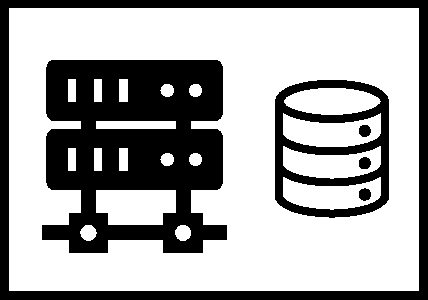
\includegraphics[width=0.4\linewidth]{images/central.pdf}
    \end{center}
    
  \end{minipage}\pause vs.\hspace{1.5em}%
  \begin{minipage}{0.5\linewidth}
    \pause
    \begin{center}
      Data collection \emph{by users} \\[0.5em]
      
      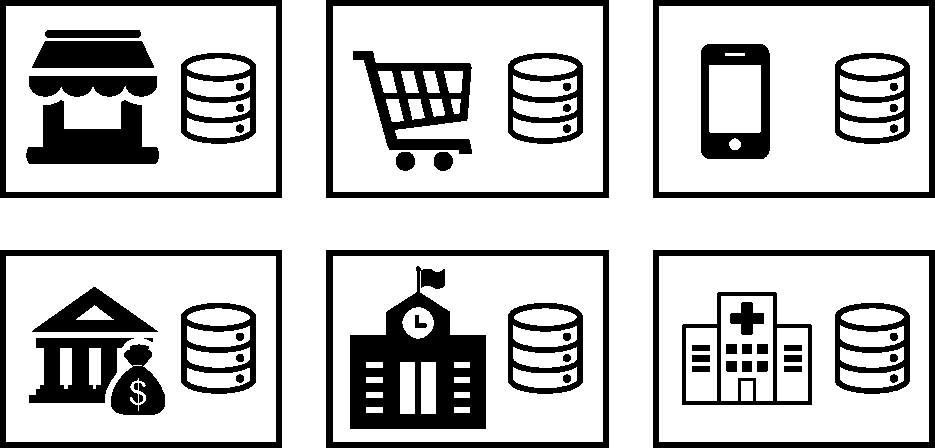
\includegraphics[width=0.8\linewidth]{images/decentralized.pdf}
    \end{center}
  \end{minipage}

  \vspace{1em}

  \pause
  
  \begin{center}
    \textbf{
    $\rightarrow$ how to use all this data?}
  \end{center}
\end{frame}


\begin{frame}[t]{Centralizing in a data center is difficult}

  Centralizing data is often impossible
  \begin{itemize}
  \item \emph{Privacy}:

    {\small
    $\rightarrow$ data may be sensitive (e.g. health records, geolocation)
    }
    \\
    ~

  \item \emph{Volume of data}:

    {\small
      $\rightarrow$ data may be large (e.g. cameras of self-driving car)
    }
    \\
    ~
    
  \item \emph{Time}:

    {\small
    $\rightarrow$ it may be needed to take decisions quickly (e.g. reinforcement learning)
    }
    
  \end{itemize}

\end{frame}

% \begin{frame}{Why share in the first place?}

%   If it is so difficult to share data... why do it?
%   \begin{itemize}
%   \item local datasets are often too small

%     {\small
%       $\rightarrow$ no statistical significance (e.g. medical study)
%     }
%     \\
%     ~
    
    
%   \item local datasets can be biased

%     {\small
%       $\rightarrow$ if a self-driving car learns in countryside, can it drive in the city?
%     }
%     \\
%     ~
    
        
%   \end{itemize}
  
% \end{frame}


\begin{frame}{Classical vs Federated Learning}
  
  \begin{minipage}{0.4\linewidth}
    \begin{center}
      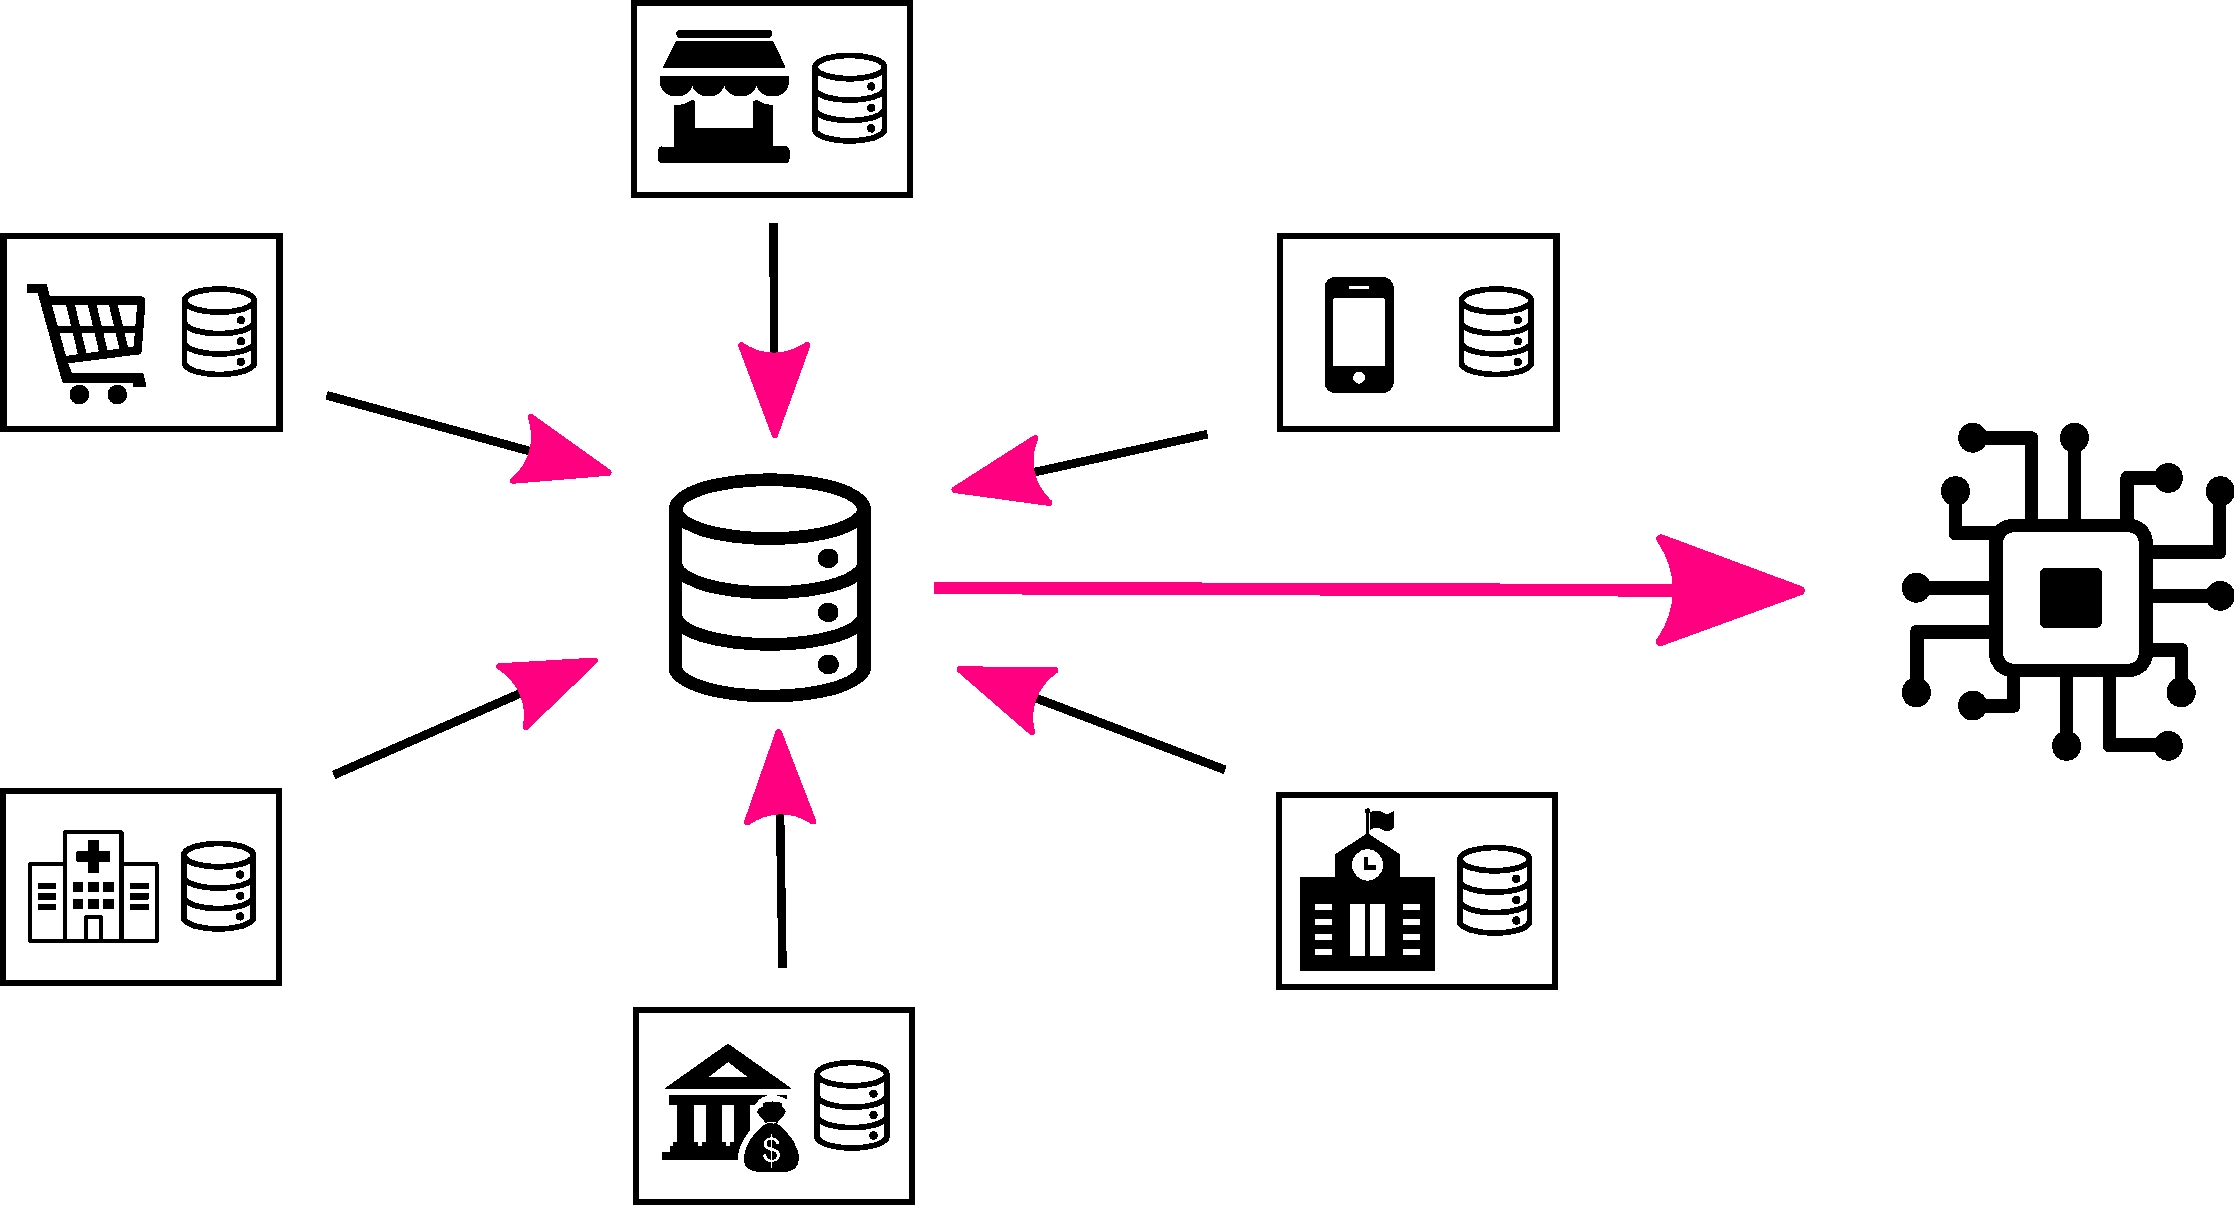
\includegraphics[width=\linewidth]{images/centralize-data.pdf}
    \end{center}
    
  \end{minipage}~~~~%
  \begin{minipage}{0.5\linewidth}
    \begin{center}
      A single optimization problem      
    \end{center}
    \begin{align*}
      \min_{\theta \in \mathbb{R}^d} \mathbb{E}_{x, y \sim D} \Big[ \ell( \theta; x, y ) \Big]
    \end{align*}
    
  \end{minipage}

\end{frame}

\begin{frame}{Classical vs Federated Learning}
  
  \begin{minipage}{0.4\linewidth}
    \begin{center}
      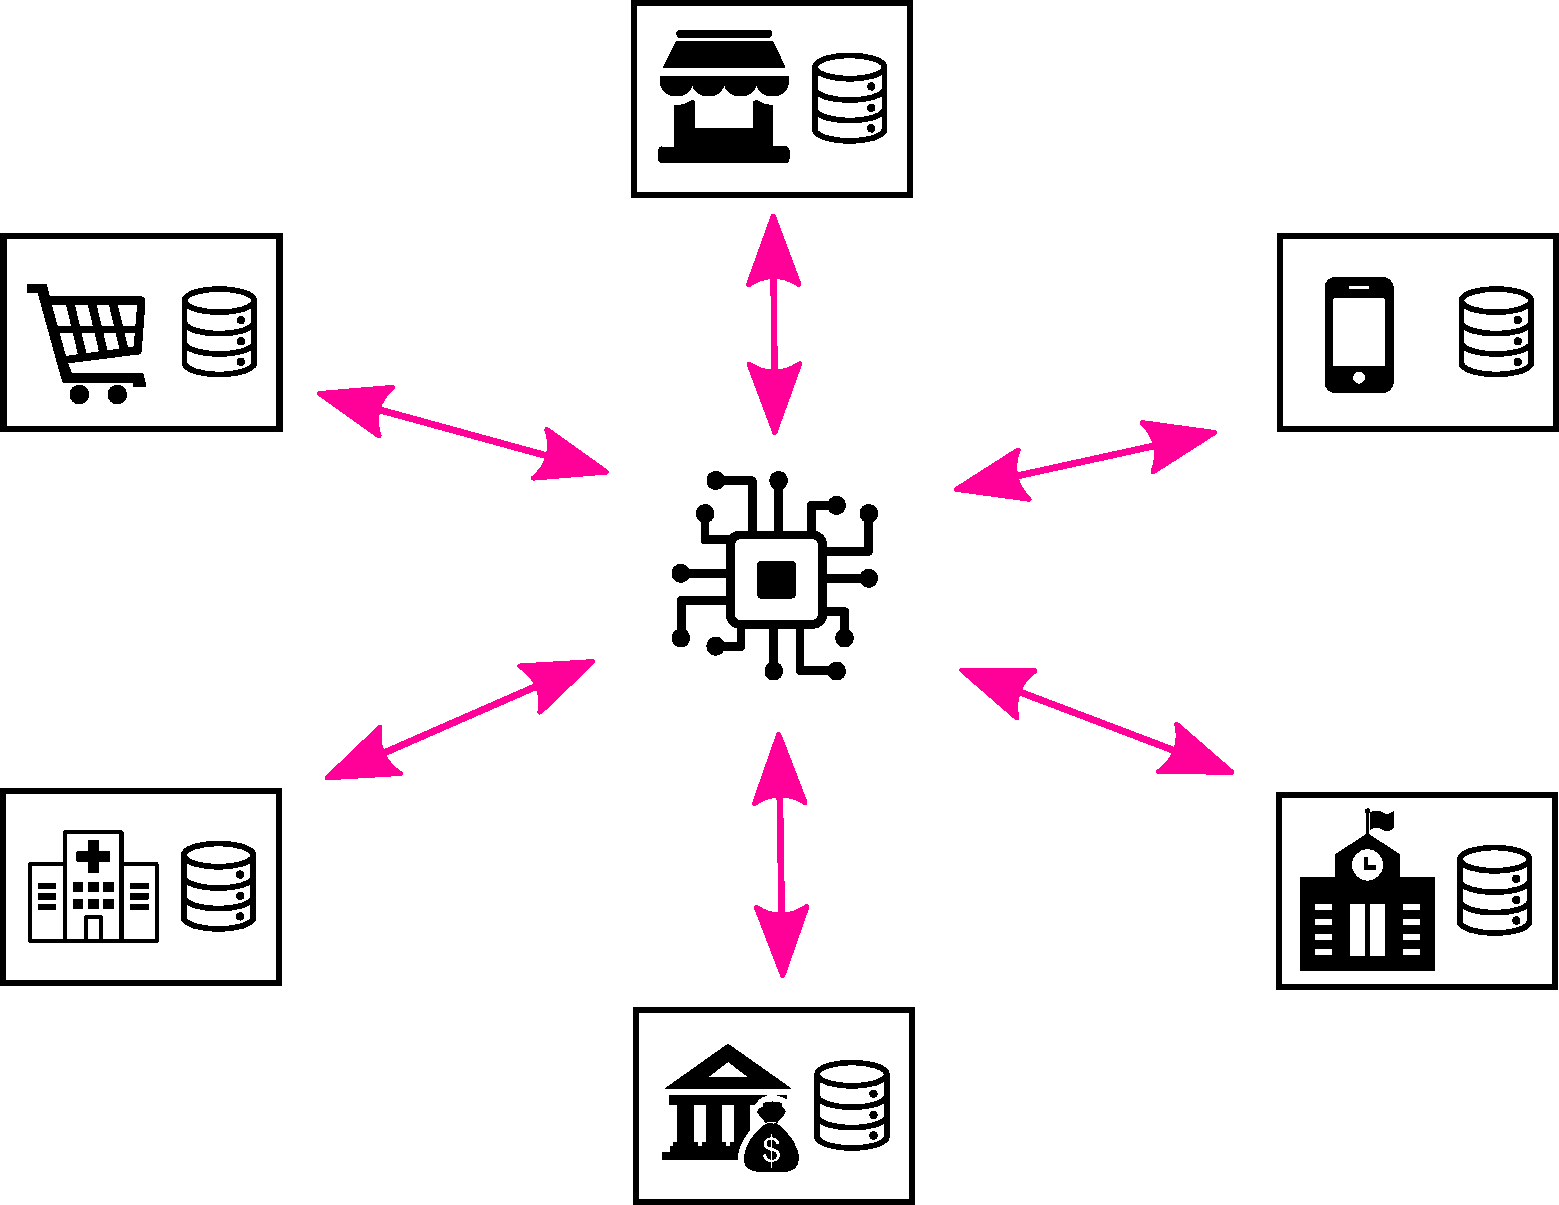
\includegraphics[width=\linewidth]{images/federated-training.pdf}
    \end{center}
    
  \end{minipage}~~~~%
  \begin{minipage}{0.5\linewidth}
    \begin{center}
      Multiple sub-problems
      \begin{align*}
        \min_{\theta \in \mathbb{R}^d} 
        \sum_{c=1}^N \mathbb{E}_{x^c, y^c \sim D^c} \Big[ \ell( \theta; x^c, y^c ) \Big]
      \end{align*}
      
      $\rightarrow$ but only \emph{one shared solution}
    \end{center}
    
  \end{minipage}


\end{frame}

\begin{frame}{Best Scenario: Homogeneous Data}

  \begin{minipage}[t]{0.5\linewidth}
    $N$ local sub-problems
    \small
    \begin{align*}
      \min_{\theta \in \mathbb{R}^d}
      \mathbb{E}_{x^1, y^1 \sim D^1} \Big[ \ell( \theta; x^1, y^1 ) \Big]
      \rightarrow
      \theta_\star^1
    \end{align*}

    \vspace{-2em}
    
    \begin{align*}
      \min_{\theta \in \mathbb{R}^d}
      \mathbb{E}_{x^2, y^2 \sim D^2} \Big[ \ell( \theta; x^2, y^2 ) \Big]
      \rightarrow
      \theta_\star^2
    \end{align*}

    \vspace{-2em}

    \begin{align*}
      \vdots
    \end{align*}

    \vspace{-2em}
    
    \begin{align*}
      \min_{\theta \in \mathbb{R}^d} 
      \mathbb{E}_{x^N, y^N \sim D^N} \Big[ \ell( \theta; x^N, y^N ) \Big]
      \rightarrow
      \theta_\star^N
    \end{align*}
  \end{minipage}~~~~%
  \begin{minipage}[t]{0.45\linewidth}
    \pause
    
    Estimate global solution
    \begin{align*}
      \theta_\star
      = \frac{1}{N} \sum_{c=1}^N \theta_\star^c
    \end{align*}

    OK if $\mathcal{D}_1 = \mathcal{D}_2 = \dots = \mathcal{D}_N$ 
  \end{minipage}
  
\end{frame}

\begin{frame}{Best Scenario: Homogeneous Data}
  \vspace{-2em}
  \begin{center}
    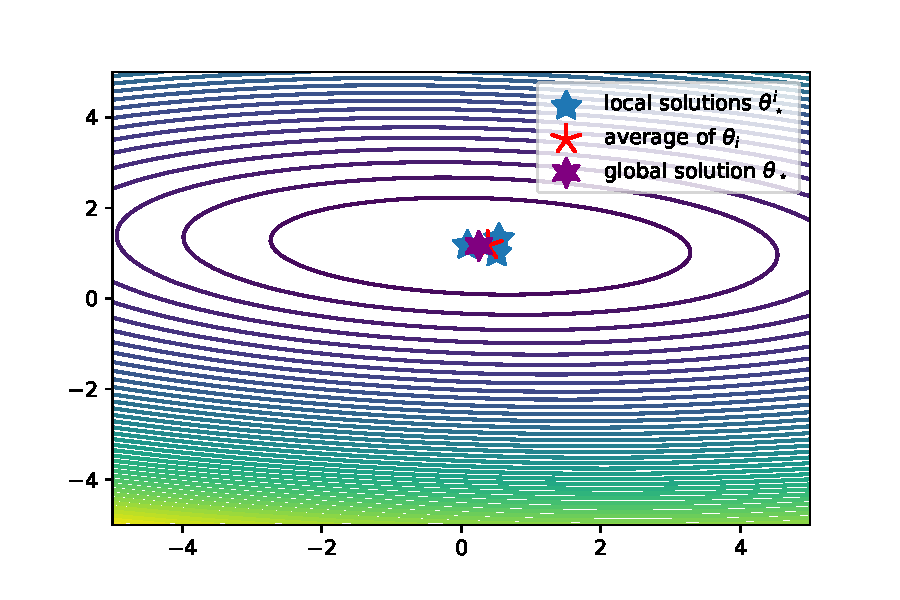
\includegraphics[width=0.8\linewidth]{images/all-minimums-homogeneous.pdf}
  \end{center}
\end{frame}

\begin{frame}{Failure: Heterogeneous Data}
  \vspace{-2em}
  \begin{center}
    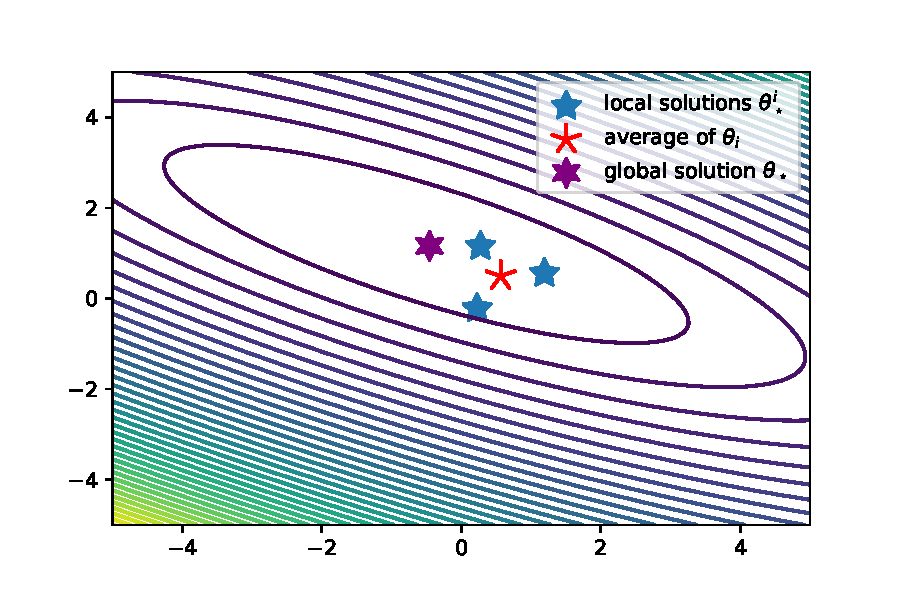
\includegraphics[width=0.8\linewidth]{images/all-minimums-heterogeneous.pdf}
  \end{center}
  \only<2>{%
    \tikz[overlay,remember picture]
    \node[fill=beamer@blendedblue!10,text=black,inner sep=2em,line width=2pt,draw=beamer@blendedblue] at ([xshift=0cm,yshift=0cm]current page.center){\LARGE We need a different method...};
  }  
\end{frame}


\begin{frame}[t]{Federated Optimization}
  \vspace{-3em}
  \begin{align*}
    \theta_\star \in \arg\min_{\theta \in \mathbb{R}^d} 
    \sum_{c=1}^N f^c(\theta)
    \enspace,
    \quad
    \text{ where }
    f^c(\theta) = \mathbb{E}_{x^c, y^c \sim D^c} \Big[ \ell( \theta; x^c, y^c ) \Big]
  \end{align*}

  \pause
  
  \vspace{-1em}

  Federated Averaging (or local (S)GD)\footfullcite{mcmahan2017communication}

  \vspace{-0.5em}
  
  \begin{itemize}
  \item For each $t = 0 ...$ :
    \begin{itemize}
      \normalsize
    \item Set $\theta_{t,0}^c = \theta_t$
    \item For each agent $c$, do $H$ gradient updates: \\[0.5em]
      
      \begin{center}
        $\theta_{t,h+1}^c = \theta_{t,h}^c - \eta \nabla f^c( \theta_{t,h}^c )$
      \end{center}
      
      \vspace{0.5em}
      
    \end{itemize}
  \item Aggregate models: $\theta_{t+1} = \frac{1}{N} \sum_{c=1}^N \theta_{t,H}^c$
  \end{itemize}

  \vspace{0.5em}

\end{frame}

%\begin{frame}{Communication and Sample Complexity\\[-0.5em]
%  \large I - Homogeneous Data}
  
%\end{frame}


%\begin{frame}{Communication and Sample Complexity\\[-0.5em]
%  \large II - Heterogeneous Data}
  
%\end{frame}

\begin{frame}{Communication and Sample Complexity\\[-0.5em]
    \large Local Training vs. Precision}
  
  \vspace{-1em}
  
  \begin{center}
    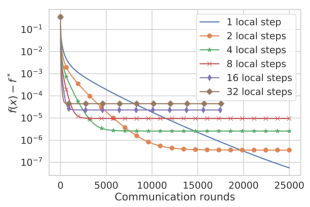
\includegraphics[width=0.6\linewidth]{images/comm-vs-local.pdf}
  \end{center}

  \vspace{-1em}

  \footnotesize
  (Figure from \fullcite{khaeld20tighter})
\end{frame}


\begin{frame}
  \begin{center}
    \textcolor{beamer@blendedblue}{
      \huge Beyond Federated Optimization:\\[0.5em]
      \huge Federated TD and LSA
    }
  \end{center}
\end{frame}


\begin{frame}{Some problems do not fit this framework...\\[-0.5em]
    \large Example: TD Learning with linear approximation (I)}

  In Federated TD learning, $N$ agent use a shared policy $\pi$ in $N$ different environments:
  \begin{align*}
    S_0^c= s, 
    A_k^c \sim \pi(\cdot | S_k^c), 
    \text{ and }
    S_{k+1}^c \sim P^c_{\text{MDP}}(\cdot| S_k^c,A_k^c)
  \end{align*}

  \pause
  
  Goal: estimate its value in each environment, for $s \in \mathcal{S}$,
  \begin{align*}
    V^{c,\pi}(s) = \textstyle{\mathbb{E}\left[\sum_{k=0}^{\infty}\gamma^{k} r^{c}(S_k^c,A_k^c)\right]}
  \end{align*}
  where $r^c$ is a reward obtained by agent $c$
\end{frame}

\begin{frame}{Some problems do not fit this framework...\\[-0.5em]
    \large Example: TD Learning with linear approximation (II)}

  Idea: build a \emph{shared estimate} of all values
  \begin{align*}
    V^{c,\pi}(s) \approx \theta^\top \varphi(s)
  \end{align*}
  using $\theta \in \mathbb{R}^d$ and embedding $\varphi: \mathcal{S} \rightarrow \mathbb{R}^d$

  \vspace{1em}
  
  \pause

  Is this meaningful to use a shared estimate? Yes, because:
  \begin{itemize}
  \item If agents are homogeneous, it reduces sample complexity
  \item If agents are heterogeneous, it may reduce bias of local data
  \end{itemize}
\end{frame}


\begin{frame}{Linear Stochastic Approximation\\[-0.5em]
  \normalsize Special case: only one agent}
  TD (with linear approx.) can be seen as solving a linear system 
  \begin{equation*}
    A \theta_\star
    = 
    b
  \end{equation*}
  where $A$ and $b$ are known through stochastic estimates $A(Z)$, $b(Z)$

  ... variance is typically very large

  \vspace{-0.5em}
  
  ... and $A$ is not symmetric
  
  \vspace{1em}

  \pause

  \small 
  Note: It is inefficient to cast it as a minimization problem with loss $\| A \theta_\star - b \|^2$\\
  $\rightarrow$ This requires a different method, with a different analysis
\end{frame}

\begin{frame}{Algorithm for LSA}
  \begin{algorithmic}
    \State Initialize $\theta_0 \in \mathbb{R}^d$
    \For{$t=0$ to $T-1$}
    \State Observe $Z_{t}$ and update:
    \begin{center}
      ~~~~~~~~~~$\theta_{t} = \theta_{t-1} - \eta( A(Z_{t}) \theta_{t-1} - b(Z_{t}))$
    \end{center}
    \EndFor
  \end{algorithmic}  
  
\end{frame}

\begin{frame}{Context, analysis of TD (I) \footfullcite{samsonov2024improved}}
  
  {\tiny
    \begin{algorithmic}
      \State Initialize $\theta_0 \in \mathbb{R}^d$
      \For{$t=0$ to $T-1$}
      \State Observe $Z^c_{t,h}$ and update: $\theta_{t} = \theta_{t-1} - \eta( A(Z_{t}) \theta_{t-1} - b(Z_{t}))$
      \EndFor
    \end{algorithmic}
  }

  \pause
  \vspace{-0.5em}
  
  \textbf{Stochastic Expansion}

  \vspace{-0.5em}

  We may write: $\theta_{t} - \theta_\star = (\text{Id} - \eta A(Z_t))(\theta_{t-1} - \theta_\star) - \eta \varepsilon(Z_t)$  

  \pause
  
  \textbf{Assumptions}

  \vspace{-0.5em}
  
  \begin{itemize}\setlength{\itemindent}{-1em}
    \small
  \item Oracle: i.i.d sequence $Z_{t}$'s such that
    $\mathbb{E} [A(Z_{t})] = A$, and
    $\mathbb{E} [b(Z_{t})] = b$
    
  \item Exponential stability: $\mathbb{E}[ \| \prod_{t=\ell}^k (\text{Id} - \eta A(Z_t)) \|^2 ] \le (1 - \eta a)^{k-\ell}$ for some $a > 0$

  \item Noise $\varepsilon(Z) = (A(Z) - A) \theta_\star + (b(Z) - b)$ has finite variance $\sigma_\star^2$
  \end{itemize}

  \vspace{1em}


\end{frame}


\begin{frame}[t]{Context, analysis of TD (II) \footfullcite{samsonov2024improved}}

  \textbf{Stochastic Expansion}
  \begin{align*}
    \theta_T - \theta_\star
    =
    \Gamma_{1:T} (\theta_0 - \theta_\star) + \eta \sum_{t=1}^T \Gamma_{t+1:T} \varepsilon(Z_t)
  \end{align*}

  Where $\Gamma_{t:t'}$ ``accumulates the updates'' from $t$ to $t'$:
  \begin{align*}
    \Gamma_{t:t'} = (\text{Id} - \eta A(Z_{t'})) (\text{Id} - \eta A(Z_{t'-1})) \cdots (\text{Id} - \eta A(Z_t))
  \end{align*}

  \vspace{1em}


\end{frame}



\begin{frame}[t]{Context, analysis of TD (III) \footfullcite{samsonov2024improved}}

  \textbf{Stochastic Expansion}
  \begin{align*}
    \theta_T - \theta_\star
    =
    \Gamma_{1:T} (\theta_0 - \theta_\star) + \eta \sum_{t=1}^T \Gamma_{t+1:T} \varepsilon(Z_t)
  \end{align*}

  \vspace{-0.5em}

  Using $\mathbb{E}[ \| \Gamma_{t:t'} u  \|^2 ] \le (1 - \eta a)^{t' - t + 1} \| u \|^2$ to bound each term:
  \begin{align*}
    \mathbb{E} [ \| \theta_T - \theta_\star \|^2 ]
    & \le
      (1 - \eta a)^T \| \theta_0 - \theta_\star \|^2
      + \frac{\eta \sigma_\star^2}{a}
  \end{align*}

  \vspace{0.5em}
  
\end{frame}


\begin{frame}{Federated LSA}
  Take $A^c, b^c$ such that $A^c \theta_\star^c = b^c$ for $c = 1 .. N$

  \pause
  
  Goal: solve collaboratively
  \begin{equation}
    \small
    \nonumber
    \Bigg( \frac{1}{N} \sum_{c=1}^{N} A^c \Bigg) \theta_\star
    = 
    \frac{1}{N} \sum_{c=1}^{N} b^c
  \end{equation}
  \vspace{-1em}

  \pause
  
  \textbf{Assumptions}

  \vspace{-0.5em}
  
  \begin{itemize}\setlength{\itemindent}{-1em}
    \small
  \item $\theta_\star$ and $\theta_\star^c$ are unique, and $A^c$ and $b^c$ are split among $N$ agents
    
  \item Oracle: i.i.d sequence $Z_{t}^c$'s such that
    $\mathbb{E} [A(Z_{t}^c)] = A^c$, and
    $\mathbb{E} [b(Z_{t}^c)] = b^c$
    
  \item Exponential stability: $\mathbb{E}[ \| \prod_{t=\ell}^k (\text{Id} - \eta A^c(Z_t^c)) \|^2 ] \le (1 - \eta a)^{k-\ell}$ for $a > 0$

  \item Noise $\varepsilon^c(Z) = (A^c(Z) - A^c) \theta_\star^c + (b^c(Z) - b^c)$ has variance bounded by $\sigma_\star^2$
  \end{itemize}

\end{frame}


\begin{frame}
  \vspace{6em}

  \begin{center}
    \textcolor{beamer@blendedblue}{
      \huge Solving Federated LSA
    }
  \end{center}

  \vspace{3em}
  

  \small
  \fullcite{mangold2024scafflsa}
\end{frame}



\begin{frame}{FedLSA Algorithm}
  \begin{algorithmic}
    \For{$t=0$ to $T-1$}
    \State Initialize $\theta_{t,0} = \theta_t$
    \For{each agent $c = 1 .. N$}
    \For{$h = 1$ to $H$}
    \State Observe $Z^c_{t,h}$ and perform local update:
    \begin{center}
      ~~~~~~~~~~$\theta_{t,h} = \theta_{t,h-1}^c - \eta( A^c(Z^c_{t,h}) \theta_{t,h-1}^c - b^c(Z^c_{t,h}))$
    \end{center}
    \EndFor
    \EndFor
    \State Aggregate local updates $\theta_{t+1} = \tfrac{1}{N} \sum\nolimits_{c=1}^{N} \theta_{t,H}^c $
    \EndFor
  \end{algorithmic}  
\end{frame}


\begin{frame}{Analysis of FedLSA}
  \textbf{Stochastic Expansion (over one communication round)}
  \begin{align*}
    \theta_{t} - \theta_\star
    & =
    \frac{1}{N} \sum_{c=1}^N \Gamma_{t,1:H}^c (\theta_{t-1} - \theta_\star)
    + \frac{1}{N} \sum_{c=1}^N (\text{Id} - \Gamma_{t,1:H}^c) (\theta_\star^c - \theta_\star)
    \\
    & \qquad + \frac{\eta}{N} \sum_{c=1}^N \sum_{h=1}^H \Gamma_{t,h+1:H}^c \varepsilon^c(Z_t^c)
  \end{align*}

  Where $\Gamma_{t,h:h'}^c$ ``accumulates local updates'', round $t$, from $h$ to $h'$,
  \begin{align*}
    \Gamma_{t,h:h'}^c = (\text{Id} - \eta A^c(Z^c_{t,h'})) (\text{Id} - \eta A^c(Z^c_{t,h'-1})) \cdots (\text{Id} - \eta A^c(Z^c_{t,h}))
  \end{align*}  
\end{frame}


\begin{frame}{Analysis of FedLSA}
  We can characterize the bias of FedLSA:
  \begin{align*}
    \theta_\infty^{\text{bias}}
    & =
      \frac{1}{N}
      \sum_{c=1}^N
      (\text{Id} - \bar{\Gamma}_{t,1:H})^{-1} 
      (\text{Id} - (\text{Id}- \eta A^c)^H)\{ \theta_\star^c - \theta_\star \}
  \end{align*}
  where $\bar{\Gamma}_{t,1:H} = \tfrac{1}{N} \sum_{c=1}^N (\text{Id} - \eta A^c)^H$

  \pause

  \vspace{1em}
  
  And give a convergence rate
  \begin{align*}
    \mathbb{E} \Big[ \| {\theta_t - \theta^{bias}_{\infty} - \theta_\star} \|^2 \Big]
    =
    O\left(
    (1 - \eta a)^{H t} \| \theta_0 - \theta_\star \|^2
    + \frac{\eta \sigma_\star^2}{N a}
    \right)
  \end{align*}
\end{frame}


\begin{frame}{Numerical Illustration}
  \vspace{-0.5em}
  
  \begin{center}
    ~~~~~Left: H=100~~~~~~~~~~~~~~~~~~~~~
    Right: H=1000
 
    \vspace{-1em}
   
    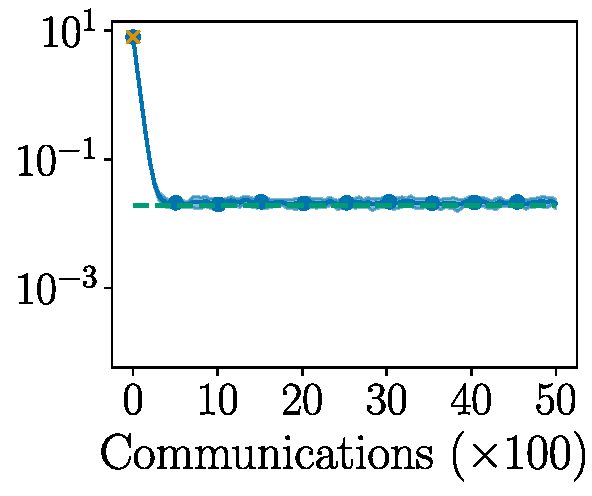
\includegraphics[width=0.4\linewidth]{images/plot_hg_100_n100_fedlsa.pdf}
    ~~
    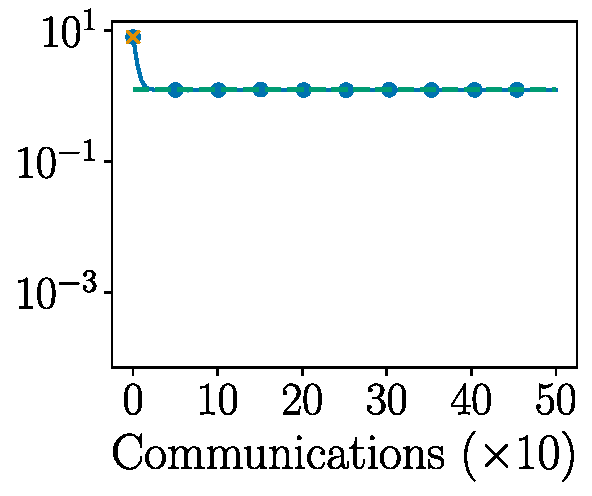
\includegraphics[width=0.4\linewidth]{images/plot_hg_1000_n100_fedlsa.pdf}
  \end{center}

  \vspace{-1em}

  Blue line: FedLSA's mean squared error

  \vspace{-1em}

  Green line: FedLSA's bias as predicted by our theory
\end{frame}


\begin{frame}{Problem: heterogeneity requires lots of communications}
  To achieve $\mathbb{E} \Big[ \| {\theta_T - \theta_\star} \|^2 \Big] \le \epsilon^2$, we need
  \begin{itemize}
  \item $\frac{\eta \sigma_\star^2}{N a} \le \epsilon^2$ ~~~~~~\,~~~~~~~~~~~~~~~~~~~ $\rightarrow$ $\eta = \frac{N a \epsilon^2}{\sigma_\star^2}$
  \item $\| \theta_T^{\text{bias}} \|^2 \le \epsilon^2$ ~~~~~~~~~~~~~~~~~~~~ $\rightarrow$ $H = \frac{\sigma_\star^2 }{N \epsilon \Delta_{\text{het}}}$
  \item $(1 - \eta a)^{H t} \| \theta_0 - \theta_\star \|^2 \le \epsilon^2$ ~~~~$\rightarrow$ $T = \frac{\Delta_{\text{het}}}{a^2 \epsilon} \log \tfrac{\| \theta_0 - \theta_\star \|}{ \epsilon }$
  \end{itemize}

  where $\Delta_{\text{het}} = \frac{1}{N} \sum_{c=1}^N \| \theta_\star - \theta_\star^c \| $
\end{frame}


\begin{frame}{Solution: Control variates (SCAFFLSA)\footnote{Based on \fullcite{karimireddy2020scaffold}}}

  \vspace{0.5em}

  \small

  \begin{algorithmic}
    \For{$t=0$ to $T-1$}
    \State Initialize $\theta_{t,0} = \theta_t$
    \For{each agent $c = 1 .. N$}
    \For{$h=1$ to $H$}
    \State Observe $Z^c_{t,h}$ and perform local update:
    \begin{center}
      ~~~~~~~~~~$\theta_{t,h} = \theta_{t,h-1}^c - \eta( A^c(Z^c_{t,h}) \theta_{t,h-1}^c - b^c(Z^c_{t,h}) - \xi_t)$
    \end{center}
  \vspace{-0.2em}
    \EndFor
  \vspace{-0.2em}
    \EndFor
    \State Aggregate local updates $\theta_{t+1} = \tfrac{1}{N} \sum\nolimits_{c=1}^{N} \theta_{t,H}^c $
    \State Update control variate $\xi_{t+1} = \xi_t - \frac{1}{\eta H} ( \theta_{t+1} - \theta_{t,H}^c )$
    \EndFor
  \end{algorithmic}
  \vspace{1.5em}
\end{frame}


\begin{frame}{Theoretical analysis}
  We prove, assuming $H \le \frac{a}{\eta \max_c \| A^c \|^2}$
  \begin{align*}
    \mathbb{E}[\| \theta_{T} - \theta_\star \|^2]
    & \lesssim{}
      \big( 
      1 - \tfrac{\eta a H}{2}
      \big)^T \psi_0
      +
      \frac{\eta \sigma_\star^2}{N a}
  \end{align*}
  with $\psi_0 = \| \theta_0 - \theta_\star \|^2 + \frac{\eta^2H^2}{N} \sum_{c=1}^N \| A^c( \theta_\star^c - \theta_\star) \|^2$


  \vspace{1em}

  \pause
  
  \small

  Note on analysis\\  
  ~~~~Direct analysis ``à la LSA'' does not work. We need a ``Lyapunov'' analysis, and to carefully study covariances of control variates to obtain linear speed-up.
\end{frame}

\begin{frame}{Numerical Illustration}
  \vspace{-0.5em}
  
  \begin{center}
    ~~~~~Left: H=100~~~~~~~~~~~~~~~~~~~~~
    Right: H=1000
 
    \vspace{-1em}
   
    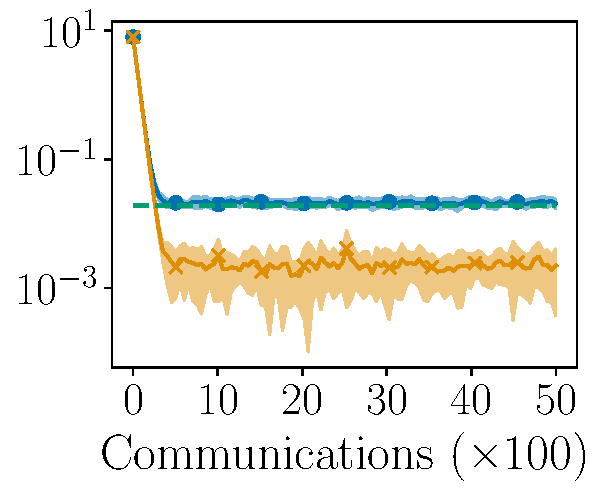
\includegraphics[width=0.4\linewidth]{images/plot_hg_100_n100.pdf}
    ~~
    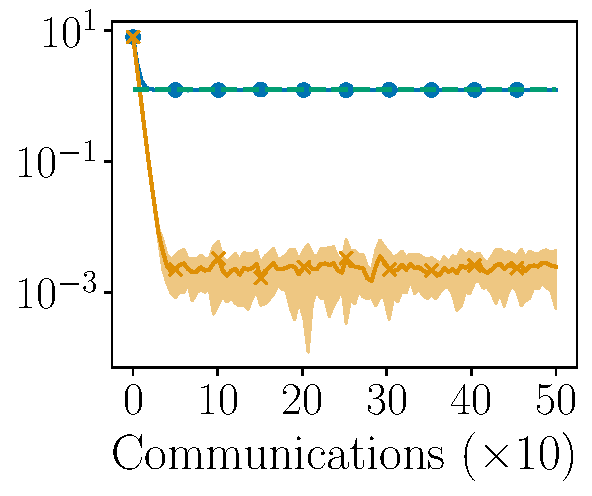
\includegraphics[width=0.4\linewidth]{images/plot_hg_1000_n100.pdf}
  \end{center}

  \vspace{-1em}

  Blue line: FedLSA's mean squared error

  \vspace{-1em}

  Orange line: SCAFFLSA's mean squared error
\end{frame}



\begin{frame}{Communication Complexity}
  To achieve $\mathbb{E} \Big[ \| {\theta_T - \theta_\star} \|^2 \Big] \le \epsilon^2$, we need
  \begin{itemize}
  \item $\frac{\eta \sigma_\star^2}{N a} \le \epsilon^2$ ~~~~~~\,~~~~~~~~~~~~~~~~~~~ $\rightarrow$ $\eta = \frac{N a \epsilon^2}{\sigma_\star^2}$
  \item $H \le \frac{a}{\eta \max_c \| A^c \|^2}$ ~~~~~~~~~~~~~~~~~ $\rightarrow$ $H = \frac{ \sigma_\star^2 }{N \epsilon^2 \max_c \| A^c \|^2}$
  \item $(1 - \frac{\eta a H}{2})^{t} \psi_0 \le \epsilon^2$ ~~~~~~~~~~~~\,~~$\rightarrow$ $T = \frac{2 \max_c \| A^c \|^2}{a^2} \log \tfrac{\psi_0}{ \epsilon }$
  \end{itemize}

  $\rightarrow$ $H \propto 1/N\epsilon^2$ rather than $1/N\epsilon$, and $T$ independent on $\epsilon$


\end{frame}

% \begin{frame}
%   \vspace{1em}

%   \begin{center}
%     Parameter setting required to reach $\mathbb{E} \left[ \| \theta_{T} - \theta_\star \|^2 \right] \le \epsilon^2 $ for different algorithms/analyses

%     \vspace{-1em}

%   \end{center}
%     \footnotesize
%     \renewcommand{\arraystretch}{1.25}
%     \centering 
%     \begin{tabular*}{0.9\textwidth}{@{\extracolsep{\fill}} cccccc }
%       % \begin{tabular}{ccccc}
%       \toprule
%         & 
%         Algorithm & 
%         Communication $T$ &
%         Local updates $H$ &
%         Sample complexity $TH$
%     \\
%     \midrule
%          & FedLSA \footfullcite{doan2020local}
%          &
%          $\displaystyle\displaystyle\mathcal{O}\left(\tfrac{N^2}{a^2 \epsilon^2} \log \tfrac{1}{\epsilon}\right)$
%          &
%          $1$
%          &
%          $\displaystyle\mathcal{O}\left(\tfrac{N^2}{a^2 \epsilon^2}\log \tfrac{1}{\epsilon}\right)$
%     \\
%     \midrule
%          ~\parbox[t]{2mm}{\multirow{3}{*}{\rotatebox[origin=c]{90}{\textbf{\textsc{ new }}}}} 
%          ~~\parbox[t]{2mm}{\multirow{3}{*}{\rotatebox[origin=c]{90}{\textbf{\textsc{ results}}}}}
%          ~
%          &
%          FedLSA %{\small [Our analysis]}
%          &
%           $\displaystyle\mathcal{O} \left({\tfrac{1}{ a^2 \epsilon}} \log{\tfrac{1}{\epsilon}} \right)$
%          &
%          $\displaystyle\mathcal{O} \bigl( \tfrac{1}{N \epsilon}\bigr)$
%          &
%          $\displaystyle\mathcal{O}\bigl(\tfrac{1}{ N a^2 \epsilon^2} \log{\tfrac{1}{\epsilon}}\bigr)$
%     \\
%         & Scaffnew \footnote{Adapted from \fullcite{mishchenko2022proxskip}} %{\small [Extended to LSA]}
%                   &
%         $\displaystyle\mathcal{O}\left(\tfrac{1}{ a \epsilon } \log \tfrac{1}{\epsilon}\right)$
%         & 
%         $\displaystyle\mathcal{O}\bigl(\tfrac{1}{a \epsilon} \bigr)$
%         &
%         $\displaystyle\mathcal{O}\bigl(\tfrac{1}{ a^2 \epsilon^2} \log{\tfrac{1}{\epsilon}}\bigr)$
%     \\
%         & Scafflsa %{\small [Our analysis]}
%                   &
%         $\displaystyle\mathcal{O}\left( \tfrac{1}{a^2} \log \tfrac{1}{\epsilon}\right)$
%         & 
%         $\displaystyle\mathcal{O}\bigl(\tfrac{1}{N \epsilon^2} \bigr)$
%         &
%         $\displaystyle\mathcal{O}\bigl(\tfrac{1}{ N a^2 \epsilon^2} \log{\tfrac{1}{\epsilon}}\bigr)$
%     \\
%     \bottomrule
%     \end{tabular*}
%     \vspace{3em}

%   \end{frame}

%   \begin{frame}{Linear Speed-Up}
%   \vspace{-0.5em}

%   MSE at stationarity (dotted line is $\propto 1/N$)

%   \vspace{-1em}
  
%   \begin{center}   
%     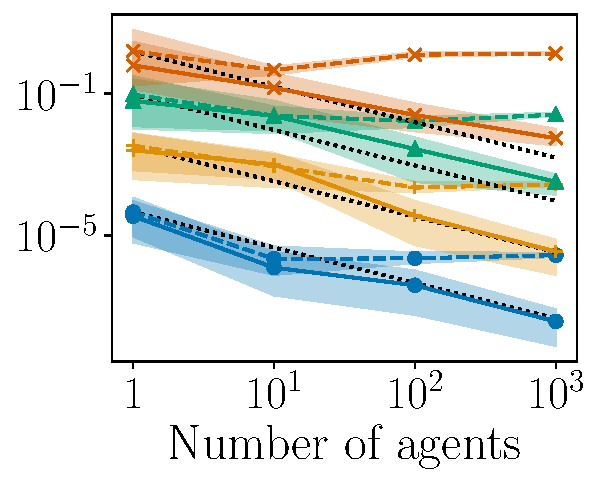
\includegraphics[width=0.5\linewidth]{images/linear-speedup.pdf}
%     
\includegraphics[width=\linewidth]{images/legend.pdf}

%     \vspace{-1.5em}

%   \end{center}

% \end{frame}

  
%\begin{frame}{Focus: linear speed-up}
  
%\end{frame}


  
  \begin{frame}
    \begin{center}
      \textcolor{beamer@blendedblue}{
        \huge What about Non-Linear?
      }
    \end{center}
  \end{frame}

  
  \begin{frame}[t]{Back to FedAvg}
    \vspace{-3em}
    \begin{align*}
      \theta_\star \in \arg\min_{\theta \in \mathbb{R}^d} 
      \sum_{c=1}^N f^c(\theta)
      \enspace,
      \quad
      \text{ where }
      f^c(\theta) = \mathbb{E}_{x^c, y^c \sim D^c} \Big[ \ell( \theta; x^c, y^c ) \Big]
    \end{align*}
    
    \vspace{-1em}

    Federated Averaging (or local (S)GD)\footfullcite{mcmahan2017communication}

    \vspace{-0.5em}
    
    \begin{itemize}
    \item For each $t = 0 ...$ :
      \begin{itemize}
        \normalsize
      \item Set $\theta_{t,0}^c = \theta_t$
      \item For each agent $c$, do $H$ gradient updates: \\[0.5em]
        
        \begin{center}
          $\theta_{t,h+1}^c = \theta_{t,h}^c - \eta \nabla f^c( \theta_{t,h}^c )$
        \end{center}
        
        \vspace{0.5em}
        
      \end{itemize}
    \item Aggregate models: $\theta_{t+1} = \frac{1}{N} \sum_{c=1}^N \theta_{t,H}^c$
    \end{itemize}

    \vspace{0.5em}

    \only<2>{%
      \tikz[overlay,remember picture]
      \node[fill=beamer@blendedblue!10,text=black,inner sep=2em,line width=2pt,draw=beamer@blendedblue] at ([xshift=0cm,yshift=0cm]current page.center){\LARGE What can we say about the bias?};
    }  

    \only<2>{\vspace{-1.8em}}%
    
  \end{frame}


  \begin{frame}{\Large For Quadratics ($f^c(\theta) = (1/2)\theta^\top A^c \theta + b \theta$)}
    The bias is the same as FedLSA
    \begin{align*}
      \theta_\infty^{\text{bias}}
      & =
        \frac{1}{N}
        \sum_{c=1}^N
        (\text{Id} - \bar{\Gamma}_{t,1:H})^{-1} 
        (\text{Id} - (\text{Id}- \eta A^c)^H)\{ \theta_\star^c - \theta_\star \}
    \end{align*}
    where $\bar{\Gamma}_{t,1:H} = \tfrac{1}{N} \sum_{c=1}^N (\text{Id}- \eta A^c)^H$

    \pause
    
    And we can give first order expansion:
    \begin{align*}
      \!\!\!\!\theta_\infty^{\text{bias}}
      & \!=\!
        \frac{\eta(H -1)}{2 N}
        \sum_{c=1}^N 
        \nabla^2 f^c(\theta_\star)^{-1} 
        (\nabla^2 f^c(\theta_\star) \!-\!  \nabla^2 f(\theta_\star)) \nabla f^c(\theta_\star)
        \!+\! O(\eta^2 H^2)
    \end{align*}
    
  \end{frame}

  \begin{frame}{In the General Case\\[-0.5em]
      \small (Strongly convex and smooth functions $f^c$)}

    Bias is in two parts!
    \begin{align*}
      \theta_\infty^{\text{bias}}
      & =
        \frac{\eta(H -1)}{2 N}
        \sum_{c=1}^N 
        \nabla^2 f^c(\theta_\star)^{-1} 
        (\nabla^2 f^c(\theta_\star) -  \nabla^2 f^c(\theta_\star)) \nabla f^c(\theta_\star)
      \\
      & \quad
        + \frac{\eta}{2 N} \nabla f^c(\theta_\star)^{-1} \nabla^3 f(\theta_\star) \textbf{A} \mathcal{C}(\theta_\star)
        + O(\eta^{3/2} + \eta^2 H^2)
    \end{align*}
    \small 
    where:

    \vspace{-1em}
    
    \begin{itemize}
    \item $\textbf{A} = (\text{Id} \otimes \nabla^2 f(\theta_\star) + \nabla^2 f(\theta_\star) \otimes \text{Id})^{-1}$
    \item  $\mathcal{C}(\theta_\star)$ is the gradient's covariance at $\theta_\star$
    \end{itemize}
    
    
  \end{frame}

  \begin{frame}{A new Federated Method?\\[-0.5em]
    \small (A bit of teasing on Richardson-Romberg)}
    \vspace{-1em}
    
    Running FedAvg with step sizes $\eta$ and $2 \eta$, we can correct the bias:

    \vspace{-1em}
    
    \begin{center}
      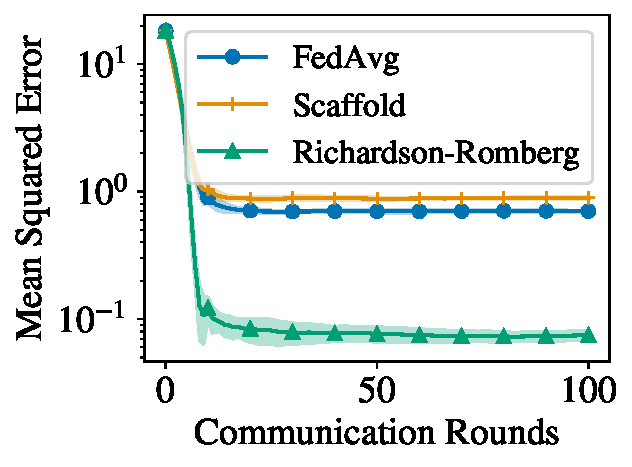
\includegraphics[width=0.5\linewidth]{images/heterogeneous_mixed_100.pdf}
    \end{center}

    \vspace{-1.5em}

    $\rightarrow$ it seems Scaffold cannot correct bias due to stochasticity!!

  \end{frame}
  
  \begin{frame}{Conclusion and Perspectives}

    \vspace{-1em}
        
    Summary:

    \vspace{-0.5em}

    \begin{itemize}
    \small      
    \item We studied FedLSA's communication complexity
    \item We extended control variates methods to FedLSA
    \item We showed that both methods have linear speed-up (up to bias)
    \item We proved first-order expansion of FedAvg's bias
    \end{itemize}

    Perspectives:

    \vspace{-0.5em}
    
    \begin{itemize}
    \small
    \item SCAFFLSA's analysis is good for small step-size: what about larger steps?
    \item Direct analysis of SCAFFLSA ``à la FedLSA''?
    \item Methods that correct all bias in non-linear regimes?
    \item Removing hyperparameters?
    \end{itemize}
  \end{frame}

  \begin{frame}
    \begin{center}
      \LARGE Thank you!

      \normalsize Questions?
    \end{center}
    

    \small
    See the paper(s):

    \fullcite{mangold2024scafflsa}

    On FedAvg and Richardson-Romberg: soon on arXiv!
  \end{frame}


\end{document}
%%% Local Variables:
%%% mode: latex
%%% TeX-master: t
%%% End:
